\documentclass{beamer}


% \usepackage{CJKnumb}\usepackage{beamerthemesplit}

\mode<article>
{
  \usepackage{beamerbasearticle}
  \usepackage{fullpage}
  \usepackage{hyperref}
}

%\usepackage{beamerthemesplit} 
%\usepackage{beamerthemeshadow}  
%\usepackage[width=2cm,dark,tab]{beamerthemesidebar}


% Setup appearance:

%\usetheme{Darmstadt}
\usefonttheme[onlylarge]{structurebold}
\setbeamerfont*{frametitle}{size=\normalsize,series=\bfseries}
\setbeamertemplate{navigation symbols}{}

\renewcommand\arraystretch{1.5}

% Standard packages

\usepackage[english]{babel}
%\usepackage[latin1]{inputenc}

\usepackage{epsf}
\usepackage{amsmath,amssymb}
\usepackage{graphicx}
\usepackage{tabularx}

% \usepackage[usenames,dvipsnames]{color}
\definecolor{shadow}{gray}{0.8}
\newcommand{\redc}[1]{{\color{red} #1}}
\newcommand{\bluec}[1]{{\color{blue} #1}}
\newcommand{\shadowc}[1]{{\color{shadow} #1}}
\definecolor{myyellow}{HTML}{FFB700}
\newcommand{\yellowc}[1]{{\color{myyellow} #1}}
\newcommand{\greenc}[1]{{\color{green} #1}}
\newcommand{\vect}[1]{\textbf{\textit{#1}}}
\renewcommand{\d}[1]{\textrm{#1}}


\usepackage{amsfonts}
\newcommand{\tickYes}{\checkmark}
\usepackage{pifont}
\newcommand{\tickNo}{\hspace{1pt}\ding{55}}

% \usetheme{Boadilla}
% \usetheme{Copenhagen}
% \usetheme{Madrid}
\usetheme{Singapore}


\begin{document}
%\title{Comparative atomistic and coarse-grained study of water: Simulation details vs. Simulation feasibility}
%\title[Optimizing SPME]{Optimizing Working Parameters of the Smooth Particle Mesh Ewald Algorithm}
\title[]{
  The numerical accuracy of force computation in inhomogeneous and correlated molecular systems.
}
%
\author{Han Wang}
\institute[FUB] {
  Institute for Mathematics, Freie Universit\"at Berlin, Germany
\vskip 0.4cm
Joint with: Christof Sch\"utte (FUB), Pingwen Zhang (PKU)}
\date[7 July 2013]{7 July 2013\\University of Edinburgh}
\frame{\titlepage}

% \begin{frame}{Why?}
%   \begin{itemize}
%     \vfill
%   \item <1-> Why force computation?
%     \begin{itemize}\itemsep 3pt
%     \item <2->Molecular dynamics simulation.
%     \item <3->Computationally intensive: \redc{$ \sim 90 \%$}
%     \item <4->One of the main sources of the \redc{``error''}.
%     \item <5->May introduce \redc{unphysical artifacts}.
%     \end{itemize}
%     \vfill
%   \item <6-> Why error estimate?
%     \begin{itemize}\itemsep 3pt
%     \item <7->Understanding \& correcting
%       the unphysical artifacts, quantitatively.
%     \item <8->Correction to force, energy, pressure, etc.
%     \item <9->Boost the efficiency of simulation automatically.
%     \end{itemize}
%     \vfill
%   \end{itemize}
% \end{frame}

\begin{frame}{Background: Molecular dynamics simulation}
  \begin{itemize}\itemsep -10pt
  \item<1-> Molecular dynamics (MD) simulation:
    \bluec{
      \begin{align*}
        m_i \frac{\d d^2\vect r_i}{\d dt^2} = \vect F_i, \quad i = 1, 2, \cdots, N
      \end{align*}
    }
  \item<2-> Pairwise interaction:
    \bluec{
      \begin{align*}
        \vect F_i = \sum_{j\neq i}\, \vect f(\vect r_i - \vect r_j)
      \end{align*}}
  \item<3-> \bluec{$\vect f$} can be:\\
    van der Waals interaction modeled by the Lennard-Jones 12-6 potential:
    \bluec{
      \begin{align*}
        \vect f(\vect r) = -\nabla_{\vect r}
        \Big(
        \frac{C_{12}}{\vert\vect r\vert^{12}}
        -\frac{C_{6}}{\vert\vect r\vert^{6}}
        \Big)
      \end{align*}
    }\\
    Electrostatic interaction modeled by the Coulomb potential:
    \bluec{
      \begin{align*}
        \vect f(\vect r) \propto -\nabla_{\vect r}
        \Big(
        \frac{1}{\vert \vect r\vert}
        \Big)
      \end{align*}}
  \end{itemize}
\end{frame}

% \begin{frame}{Motivation of our study}
%   Why force computation is important?
%   \begin{itemize}\itemsep 3pt
%   \item <2->Computationally intensive: \redc{$ \sim 90 \%$}
%   \item <3->One of the main sources of the \redc{``error''}.
%   \item <4->May introduce \redc{unphysical artifacts}.
%   \end{itemize}
%   \vfill
% \end{frame}


\begin{frame}{Fast algorithms of the force computation}
  \begin{itemize}
  \item<1-> Naive solution:
    \bluec{
      \begin{align*}
        \vect F_i = \sum_{j=1,j\neq i}^N\, \vect f(\vect r_i - \vect r_j), \quad i=1,2,\cdots,N
      \end{align*}}
    costs \redc{$\mathcal O(N^2)$}
    \vfill
  \item<2-> Fast algorithms:
    \begin{itemize}
    \item<3->
      \begin{minipage}[t]{0.48\linewidth}
        \vskip -.25cm
        Lennard-Jones 12-6 \bluec{$\propto 1/r^6$}\\
        \redc{Cut-off method\quad $\mathcal O(N)$}        
      \end{minipage}
      \begin{minipage}[t]{0.48\linewidth}
        \vskip -1.5cm
        \begin{figure}
          \centering 
          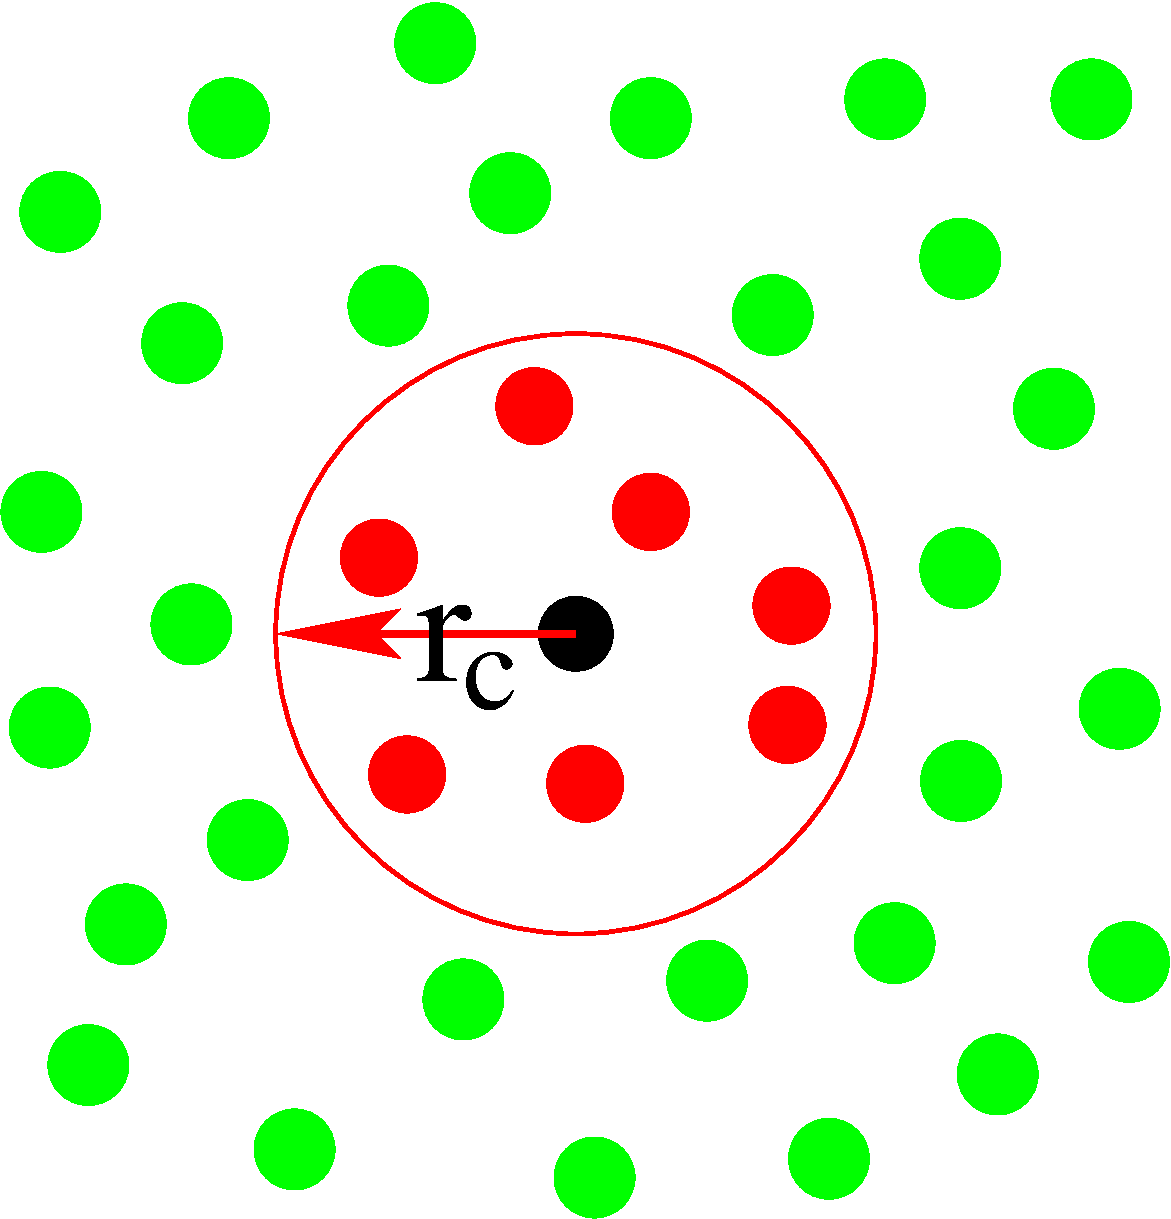
\includegraphics[width=0.8\textwidth]{figs/short-range/simple-cutoff.pdf}
        \end{figure}        
      \end{minipage}
    \item<4->
      Coulomb \bluec{$\propto 1/r$}\\
      \redc{Smooth Particle Mesh Ewald (SPME) method\\
        $\mathcal O(N \log N)$}
    \end{itemize}
  \end{itemize}
\end{frame}


\begin{frame}{Cut-off in homogeneous systems}
  \begin{itemize}
  \item<1-> However, there is \redc{NO} free lunch... Error of force.
  \item<2-> Expense: \redc{$\mathcal O(r_c^3)$}. Force computation costs \redc{$ \sim 90 \%$} of a typical molecular dynamics simulation.
  \item<3-> Mostly used $r_c$: 2.5 -- 4.0 $\sigma$ for homogeneous systems.
  \item<4->\redc{Convergence check} needed (in extreme cases).
  \begin{figure}
      \centering
      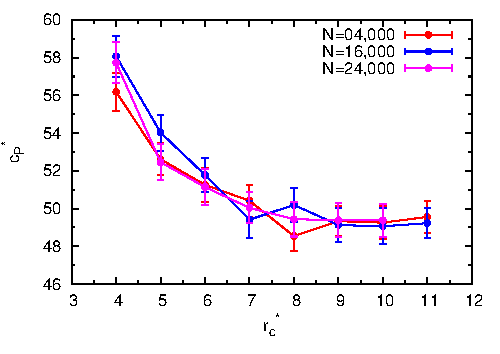
\includegraphics[width=0.6\textwidth]{figs/simple-cut-conv/natom-rcut-c.pdf}
    \end{figure}
  \end{itemize}
\end{frame}


\begin{frame}{Unphysical cut-off artifacts due to inhomogeneity}
  \begin{itemize}\itemsep 10pt
  \item<1-> Example system:
    \begin{figure}
      \centering
      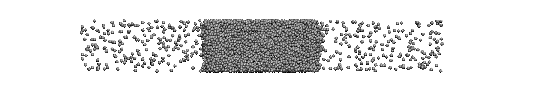
\includegraphics[width=0.9\textwidth]{figs/t0.85-n16000-rc07.5uni/confout-02.eps}
    \end{figure}
  \item<2-> Equilibrium densities:
    \begin{figure}
    \centering
    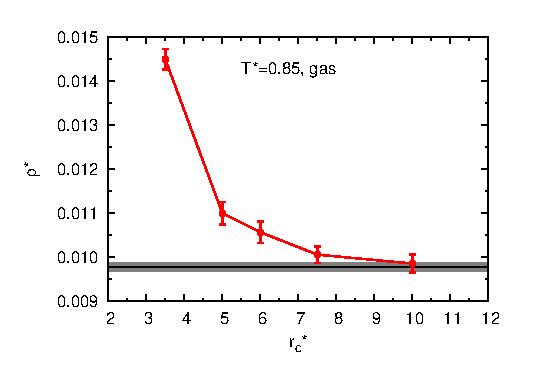
\includegraphics[width=0.49\textwidth]{figs/converge.new/t0p85-gas-1.eps} 
    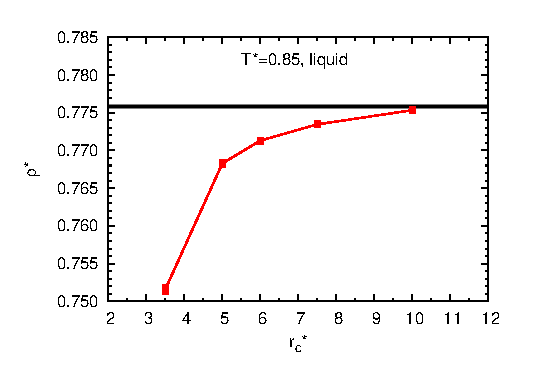
\includegraphics[width=0.49\textwidth]{figs/converge.new/t0p85-liquid-1.eps} 
  \end{figure}  
  \end{itemize}
\end{frame}

\begin{frame}{One more example}{Surface tension of 61 organic liquids}
  \begin{figure}
    \centering
    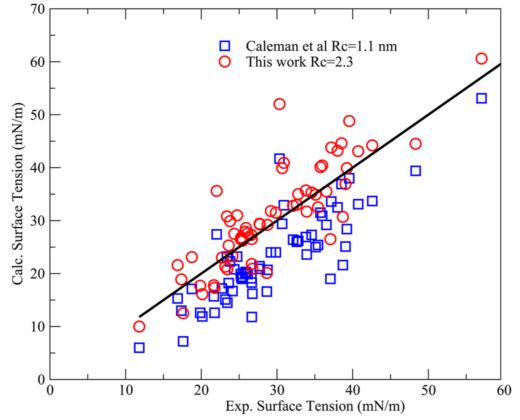
\includegraphics[width=0.6\textwidth]{figs/short-range/membrane-example.pdf} 
  \end{figure}
  \bluec{R.A. Zubillaga et. al., Journal of Chemical Theory and Computation, in press, 2013}
\end{frame}

\begin{frame}{Motivation of quantitative error study}
  \redc{How much error do we produce by using a fast algorithm?}
  \\
  \vskip 1cm
  
  What can we do by estimating the error?
  \begin{itemize}\itemsep 3pt
  \item <2->Understanding
    the unphysical artifacts, quantitatively.
  \item <3->Cheap correction to density, energy, pressure, etc.
  \item <4->Boost the accuracy \& efficiency of simulation automatically.
  \end{itemize}  
  \vfill
\end{frame}



\begin{frame}{Definition of force error}
  \begin{itemize}
  \item<1->   The difference between exact force and computed force by fast algorithms:
  \bluec{
    \begin{align*}
      \Delta \vect F(\vect r)
      &=
      \vect F_{\textrm{exact}}(\vect r) - \vect F_{\textrm{calculate}}(\vect r) 
    \end{align*}
  }
  which is called \redc{error force}.
  \vskip .5cm
  \item<2-> Error of a fast algorithm: 
  \bluec{
    \begin{align*}
      \mathcal E =\sqrt{ \langle\vert\Delta\vect F(\vect r)\vert^2\rangle}
    \end{align*}
    }
  \end{itemize}
\end{frame}



% \begin{frame}{The working parameters of SPME} {A 6 dimensional parameter space!}
%   \begin{figure}
%     \centering
%     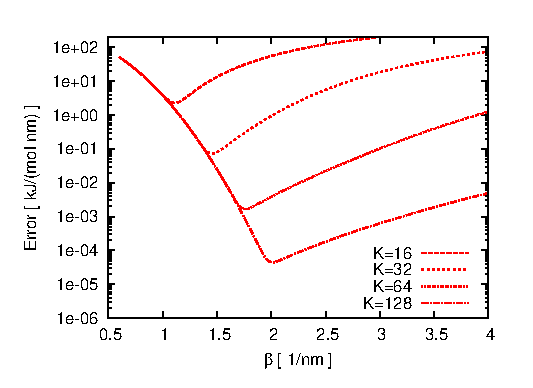
\includegraphics[width=0.9\textwidth]{figs/long-range/error-uniform.eps}
%   \end{figure}  
% \end{frame}

\begin{frame}{Overview of the error estimates}
  \begin{itemize}
  \vfill
  \item<1->   Conditions for the error estimate:
  \begin{enumerate}\itemsep 3pt
  \item \redc{Homogeneous}.
  \item Particles are \redc{uncorrelated}.
  \end{enumerate}
  \vfill
\item<2->   Current error estimates:
  \begin{table}
    \centering
    \begin{tabular*}{0.85\textwidth}{l@{\extracolsep{\fill}}ll}\hline\hline
      Conditions & cut-off & SPME \\\hline
      1+2 & \bluec{\tickYes\quad$\mathcal O(1)$}  & \bluec{\tickYes\quad$\mathcal O(1)$} \\
      2   & \redc{\tickYes\quad$\mathcal O(N\log N)$} & \redc{\tickYes\quad$\mathcal O(N\log N)$} \\
      none& \redc{\tickNo\quad$\mathcal O(N^2\log N)$} & \redc{\tickNo\quad$\mathcal O(N^2\log N)$} \\
          &  & \redc{N.N.A. $\mathcal O(N\log N)$} \\\hline\hline
    \end{tabular*}
  \end{table}
  \vfill
  \end{itemize}
\end{frame}

\begin{frame}{Short-range, homogeneous, uncorrelated}
  \begin{enumerate}\itemsep 3pt
  \item {Homogeneous}.
  \item Particles are {uncorrelated}.
  \end{enumerate}
    \begin{table}
    \centering
    \begin{tabular*}{0.85\textwidth}{l@{\extracolsep{\fill}}ll}\hline\hline
      Conditions & cut-off & SPME \\\hline
      1+2 & \bluec{\tickYes\quad$\mathcal O(1)$}  & \shadowc{\tickYes\quad$\mathcal O(1)$} \\
      2   & \shadowc{\tickYes\quad$\mathcal O(N\log N)$} & \shadowc{\tickYes\quad$\mathcal O(N\log N)$} \\
      none& \shadowc{\tickNo\quad$\mathcal O(N^2\log N)$} & \shadowc{\tickNo\quad$\mathcal O(N^2\log N)$} \\
          &  & \shadowc{N.N.A. $\mathcal O(N\log N)$} \\\hline\hline
    \end{tabular*}
  \end{table}
\end{frame}


\begin{frame}{Short-range, homogeneous, uncorrelated}
  \begin{itemize}\itemsep -10pt
    \vfill
  \item<1-> Error estimate:
    \bluec{
      \begin{align*}
        \mathcal E^2(r_c) = 4\pi\rho\int_{r_c}^\infty r^2[u'(r)]^2 \,\d dr,
      \end{align*}}
    where \bluec{$u(r)$} is the pairwise interaction potential.
    \vfill
    \vskip 1.cm
  \item<2-> Homogeneity $\Rightarrow$ \bluec{$\langle\Delta\vect F\rangle = 0$}
    \bluec{
      \begin{align*}
        \mathcal E^2 = \textrm{Var}(\Delta\vect F)
      \end{align*}
    }
    \vfill
  \end{itemize}
\end{frame}


\begin{frame}{Short-range, inhomogeneous, correlated}
  \begin{enumerate}\itemsep 3pt
  \item {Homogeneous}.
  \item Particles are {uncorrelated}.
  \end{enumerate}
    \begin{table}
    \centering
    \begin{tabular*}{0.85\textwidth}{l@{\extracolsep{\fill}}ll}\hline\hline
      Conditions & cut-off & SPME \\\hline
      1+2 & \shadowc{\tickYes\quad$\mathcal O(1)$}  & \shadowc{\tickYes\quad$\mathcal O(1)$} \\
      2   & \redc{\tickYes\quad$\mathcal O(N\log N)$} & \shadowc{\tickYes\quad$\mathcal O(N\log N)$} \\
      none& \redc{\tickNo\quad$\mathcal O(N^2\log N)$} & \shadowc{\tickNo\quad$\mathcal O(N^2\log N)$} \\
          &  & \shadowc{N.N.A. $\mathcal O(N\log N)$} \\\hline\hline
    \end{tabular*}
  \end{table}
\end{frame}


\begin{frame}{The error estimate}
  \begin{itemize}
  \item <1-> Define the error force kernel
    \bluec{
      \begin{align*}
        \Delta \vect F(\vect r)
        &=
        q \sum_{j=1}^N q_j \,\vect K(\vect r, \vect r_j)
      \end{align*}}
    It is possible for most main stream fast force calculation algorithms: cut-off, SPME, P3M, etc.
  \item <2-> The kernel of cut-off method:
    \bluec{
      \begin{align*}
        \vect K(\vect r,\vect r') =
        \left\{
          \begin{array}{ll}
            0, & \vert\vect r - \vect r'\vert\leq r_c; \\
            \vect f(\vert\vect r-\vect r'\vert), & \vert\vect r - \vect r'\vert > r_c.
          \end{array}
        \right.
      \end{align*}}
    \vfill
  \end{itemize}
\end{frame}

\begin{frame}{The error estimate}
  \begin{itemize}\itemsep -10pt
  \item<1->   The mean error force is
    \bluec{
      \begin{align*}
        \langle\Delta\vect F(\vect r)\rangle
        =
        q\int_{\mathbb R^3}\vect K(\vect r , \vect r')\,\rho_q(\vect r')\,\d d\vect r'
      \end{align*}
    }
  \vskip -10cm
\item<2->   The error:
  \bluec{
    \begin{align*} \nonumber
      % \langle\vert\Delta\vect F(\vect r)\vert^2\rangle
      \mathcal E^2
      = 
      \redc{\mathcal E^2_{\textrm{homo}}(\vect r)} +
      % \langle\Delta\vect F(\vect r)\,\rangle^2 +
      \redc{\mathcal E^2_{\textrm{inhomo}}(\vect r)} +
      \redc{\mathcal E_{\textrm{correlation}}(\vect r)}.
    \end{align*}
  }
  with\bluec{
  \begin{align*}
    \redc{\mathcal E^2_{\textrm{homo}}(\vect r)}
    = &\,
    q^2\int_{\mathbb R^3}\vert\vect K(\vect r, \vect r')\vert^2\rho_{q^2}(\vect r')\,\d d\vect r'  \\
    \redc{\mathcal E^2_{\textrm{inhomo}}(\vect r)}
    = &\,
    q^2\bigg[\int_{\mathbb R^3}\vect K(\vect r, \vect r')\rho_q(\vect r')\,\d d\vect r'\,\bigg]^2
    \redc{ = \langle\Delta\vect F(\vect r)\,\rangle^2}
    \\
    \redc{\mathcal E_{\textrm{correlation}}(\vect r)}
    =&\,
    q^2\int_{\mathbb R^3\times\mathbb R^3}\vect K(\vect r, \vect r')\cdot\vect K(\vect r, \vect r'')\,C_{q^2}(\vect r', \vect r'')\,\d d\vect r'\d d\vect r''
  \end{align*}}
  \end{itemize}
\end{frame}


\begin{frame}{Liquid-vapor equilibrium of Lennard-Jones particles}
  \begin{figure}
    \centering
    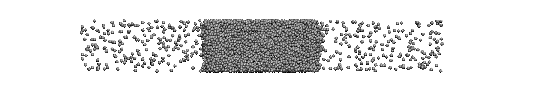
\includegraphics[scale=1]{figs/t0.85-n16000-rc07.5uni/confout-02.eps}\\
    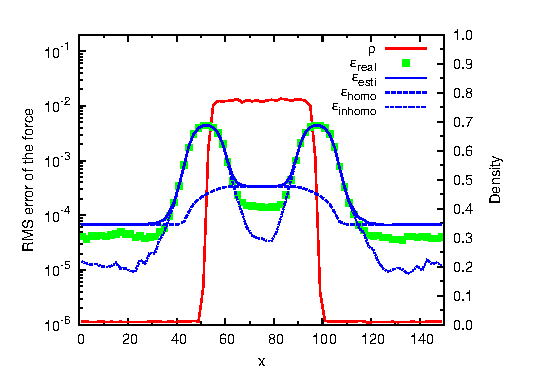
\includegraphics[]{figs/t0.85-n16000-rc07.5uni/error-uniform.eps}
  \end{figure}
\end{frame}

\begin{frame}{cut-off in bulk}
  \begin{figure}
    \centering
    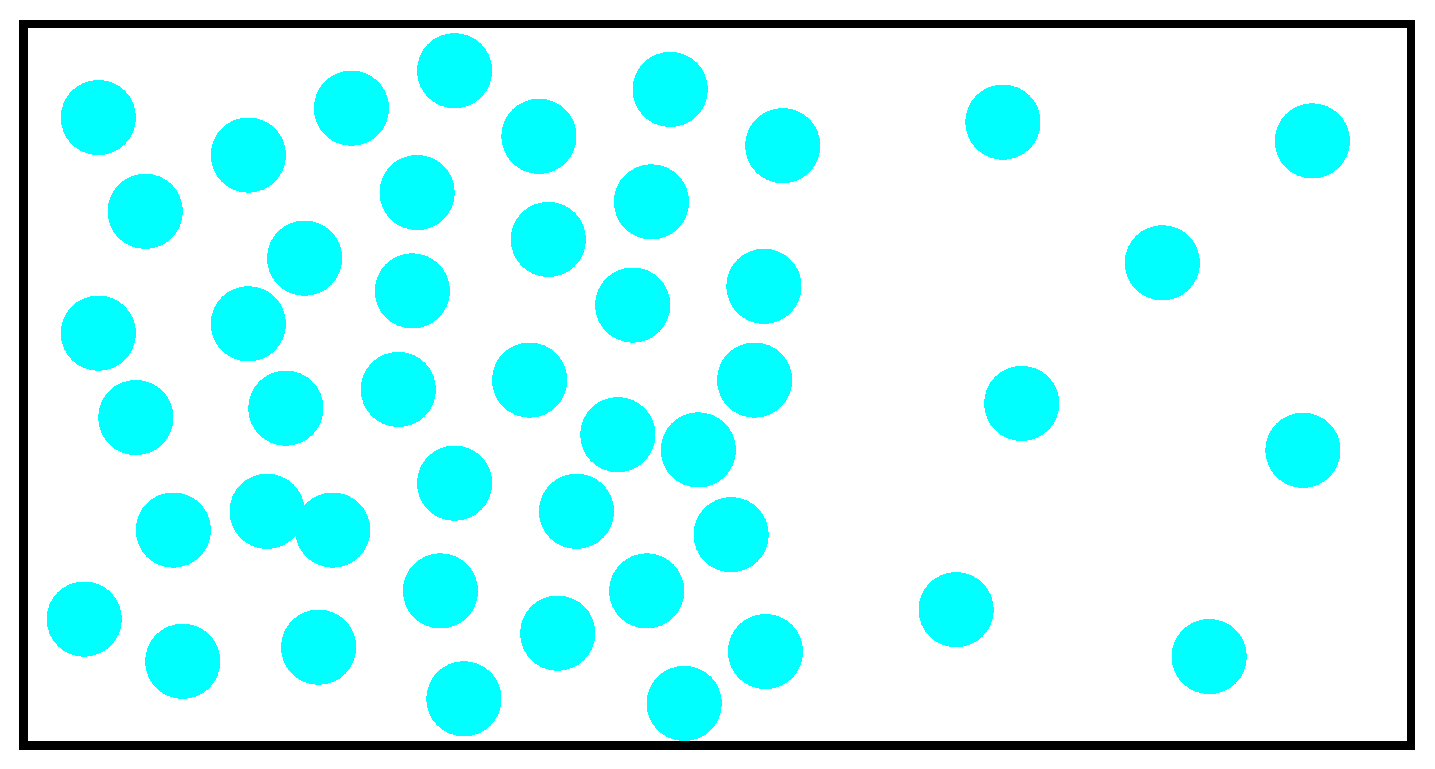
\includegraphics[width=0.9\textwidth]{figs/t0.85-n16000-rc07.5uni/cut-bulk-step00.eps}
  \end{figure}  
\end{frame}

\begin{frame}{cut-off in bulk}
  \begin{figure}
    \centering
    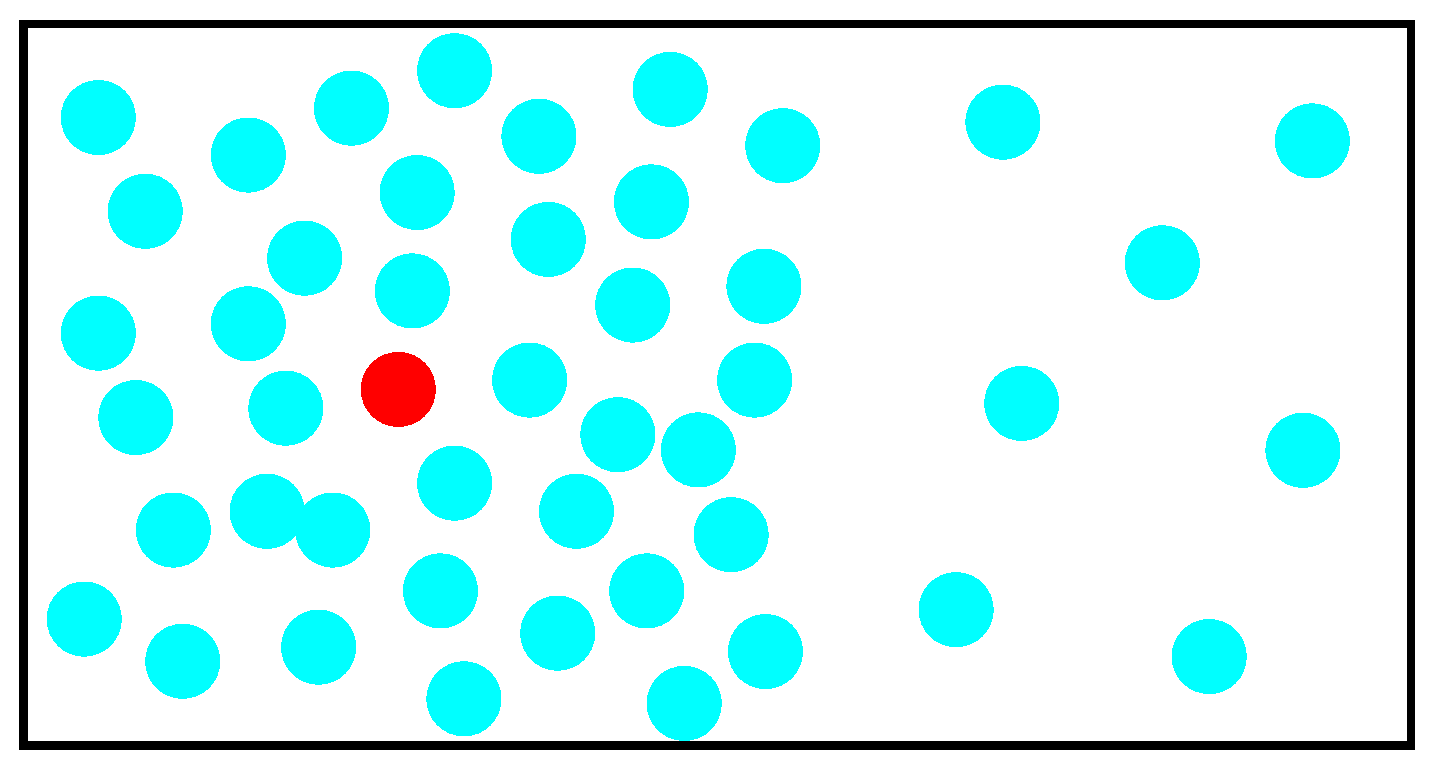
\includegraphics[width=0.9\textwidth]{figs/t0.85-n16000-rc07.5uni/cut-bulk-step01.eps}
  \end{figure}  
\end{frame}

\begin{frame}{cut-off in bulk}
  \begin{figure}
    \centering
    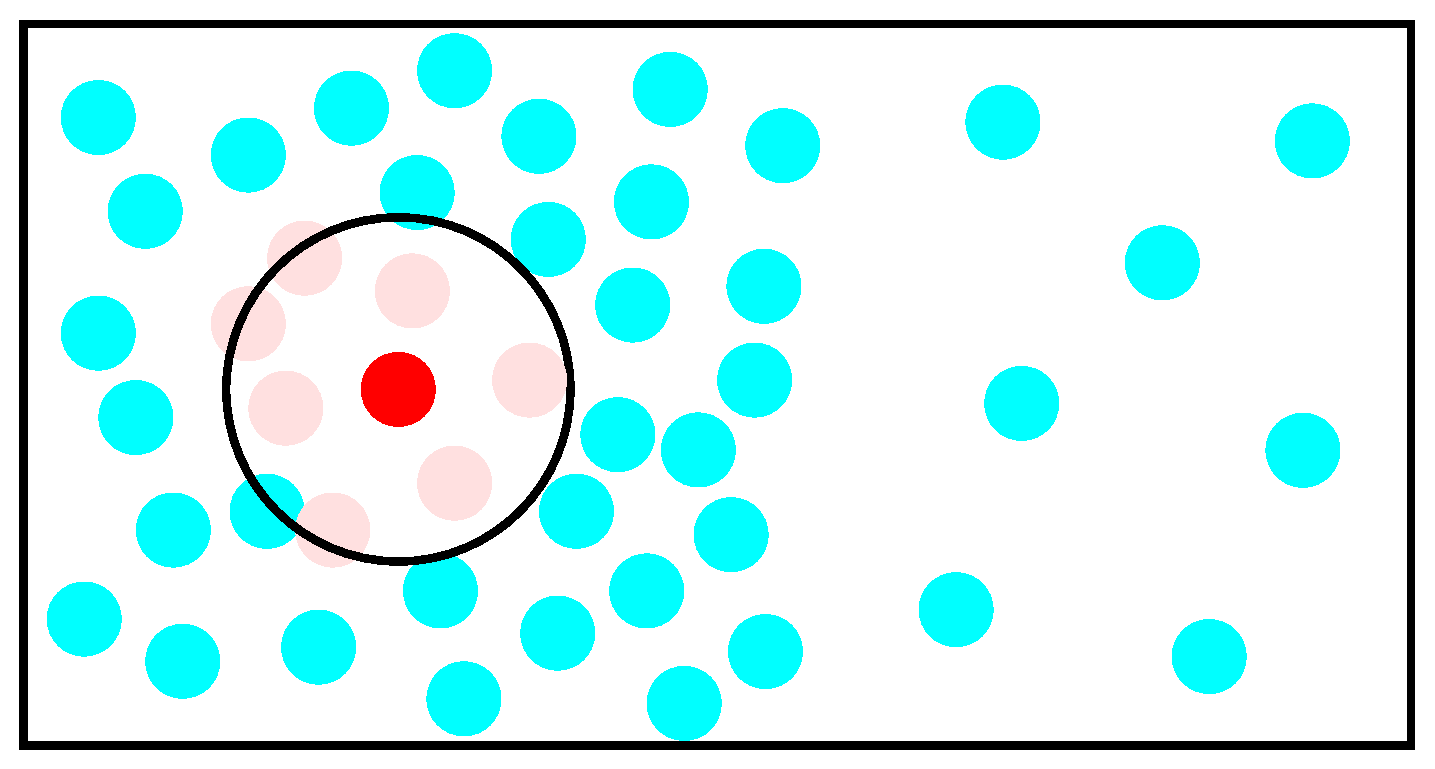
\includegraphics[width=0.9\textwidth]{figs/t0.85-n16000-rc07.5uni/cut-bulk-step02.eps}
  \end{figure}  
\end{frame}

\begin{frame}{cut-off in bulk}
  \begin{figure}
    \centering
    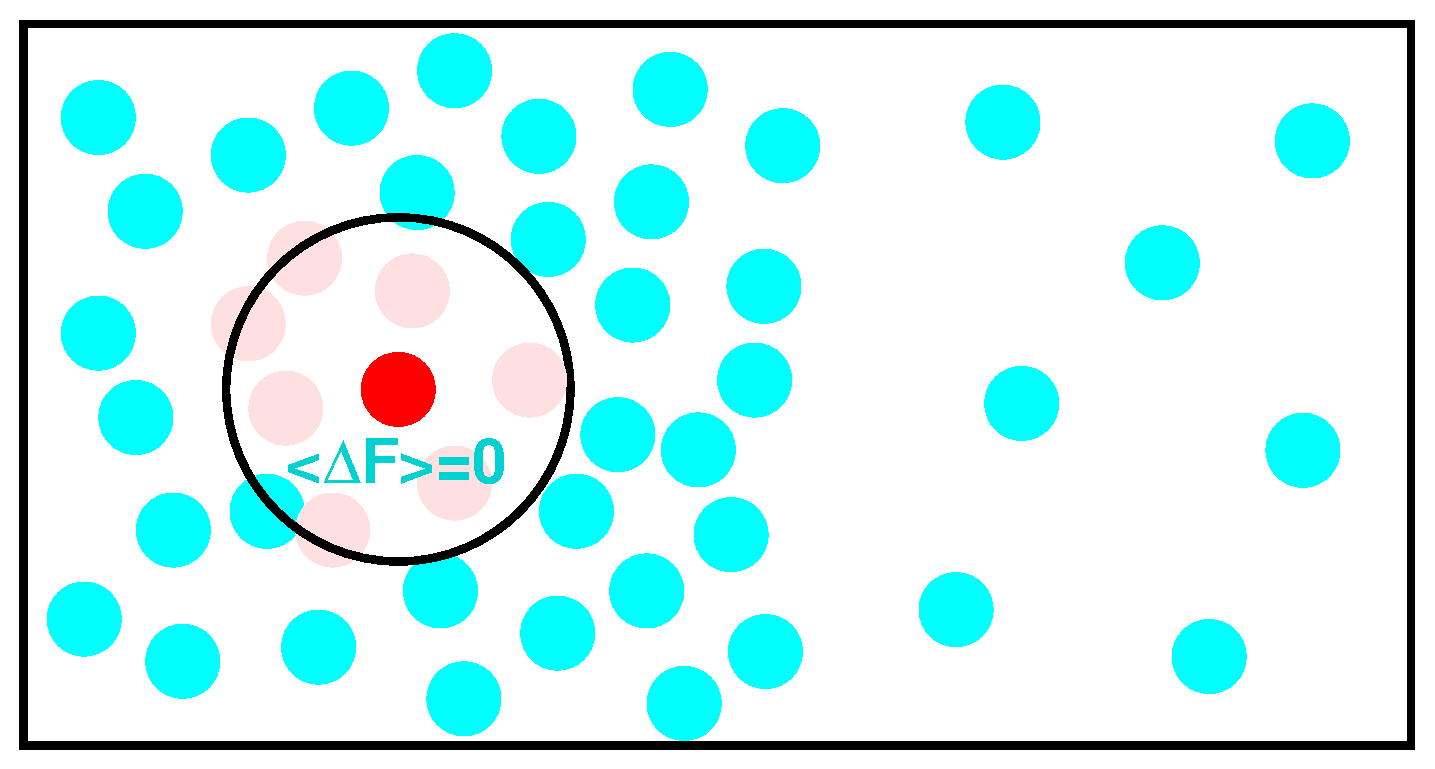
\includegraphics[width=0.9\textwidth]{figs/t0.85-n16000-rc07.5uni/cut-bulk-step03.eps}
  \end{figure}  
\end{frame}


\begin{frame}{cut-off at interface}
  \begin{figure}
    \centering
    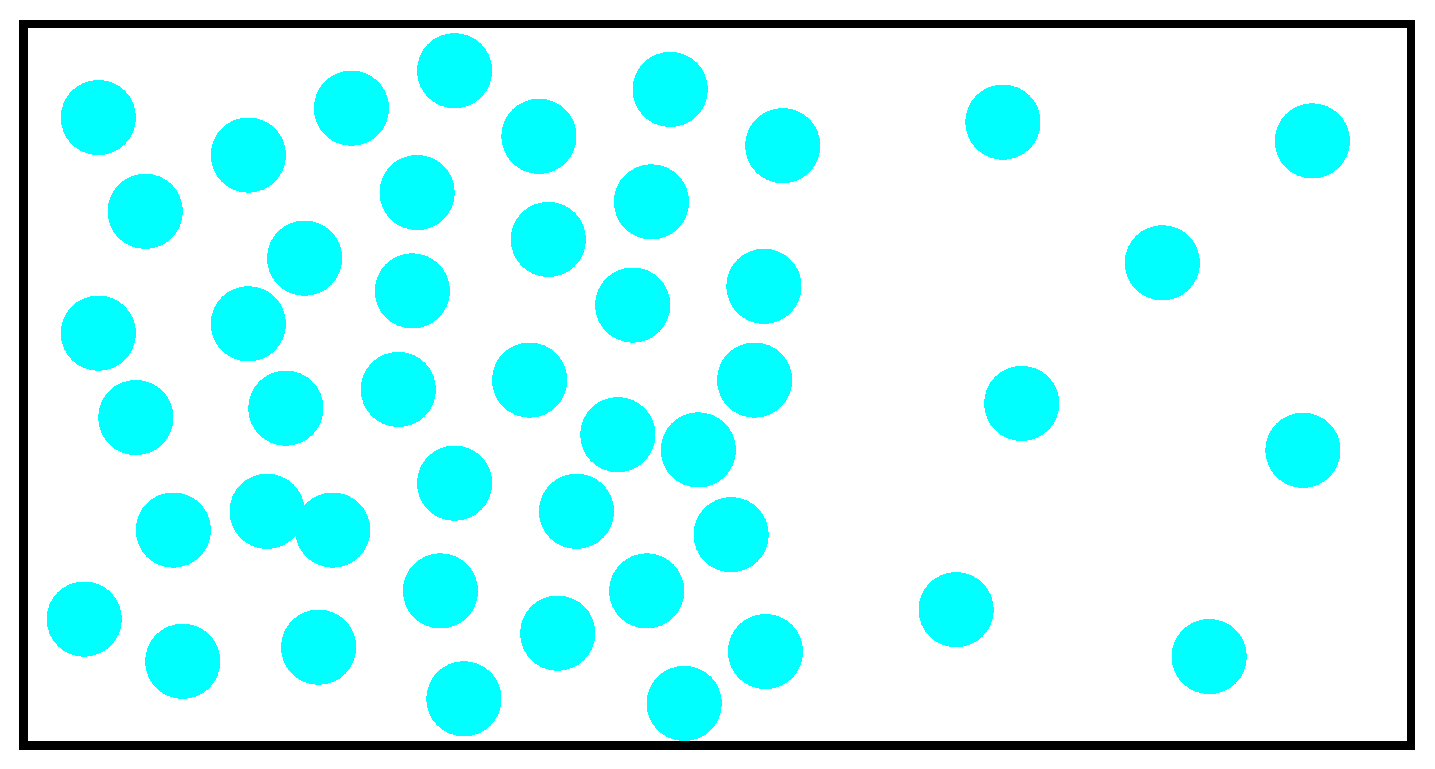
\includegraphics[width=0.9\textwidth]{figs/t0.85-n16000-rc07.5uni/cut-bulk-step00.eps}
  \end{figure}  
\end{frame}


\begin{frame}{cut-off at interface}
  \begin{figure}
    \centering
    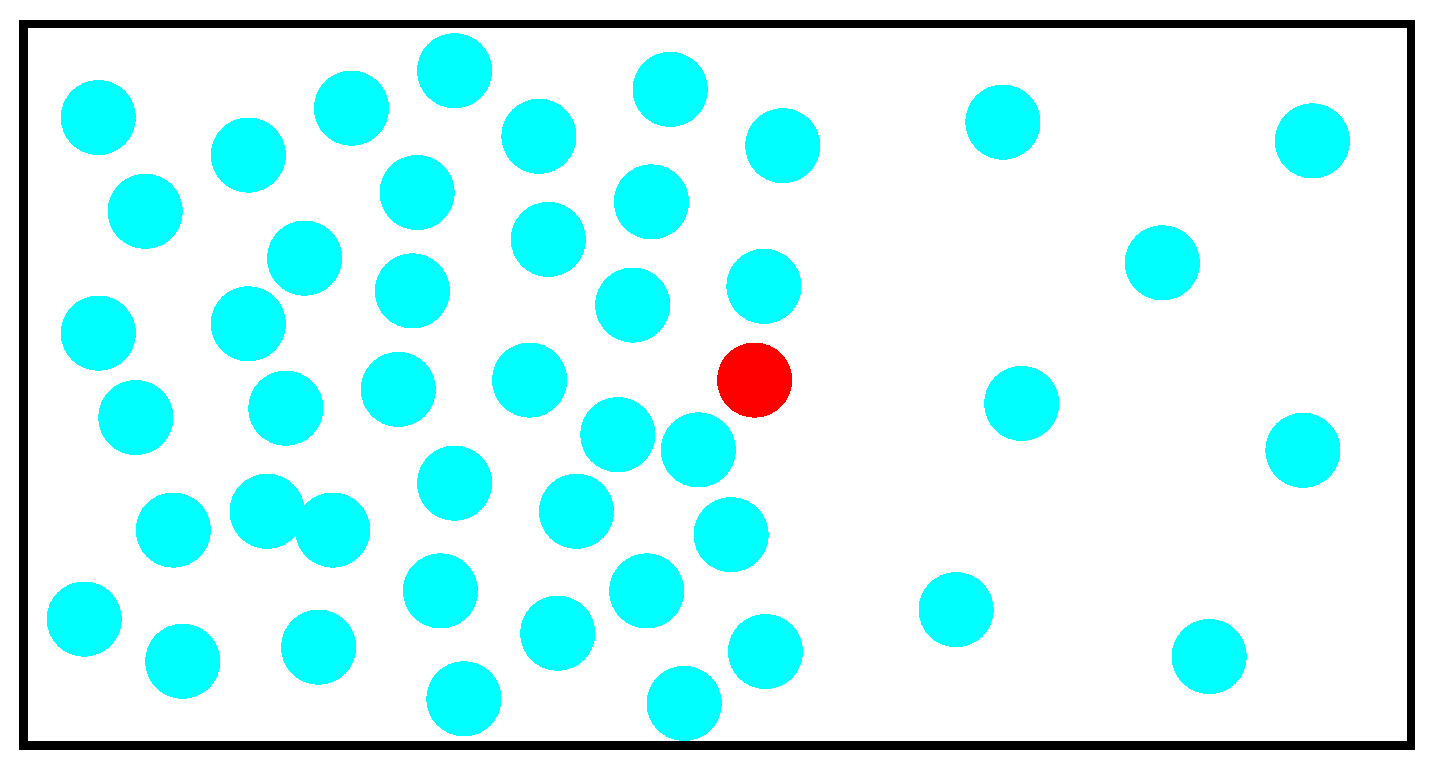
\includegraphics[width=0.9\textwidth]{figs/t0.85-n16000-rc07.5uni/cut-interface-step03.eps}
  \end{figure}  
\end{frame}


\begin{frame}{cut-off at interface}
  \begin{figure}
    \centering
    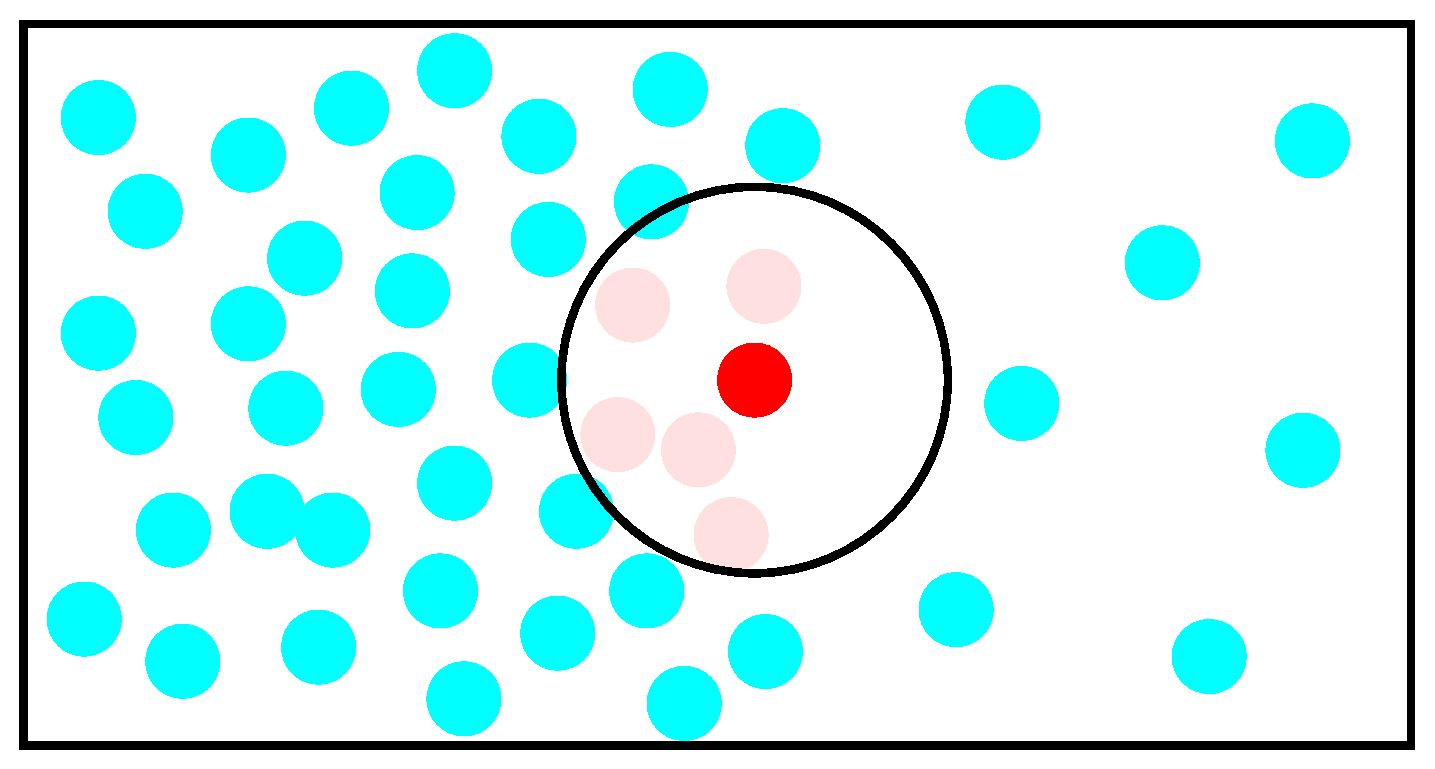
\includegraphics[width=0.9\textwidth]{figs/t0.85-n16000-rc07.5uni/cut-interface-step04.eps}
  \end{figure}  
\end{frame}

\begin{frame}{cut-off at interface}
  \begin{figure}
    \centering
    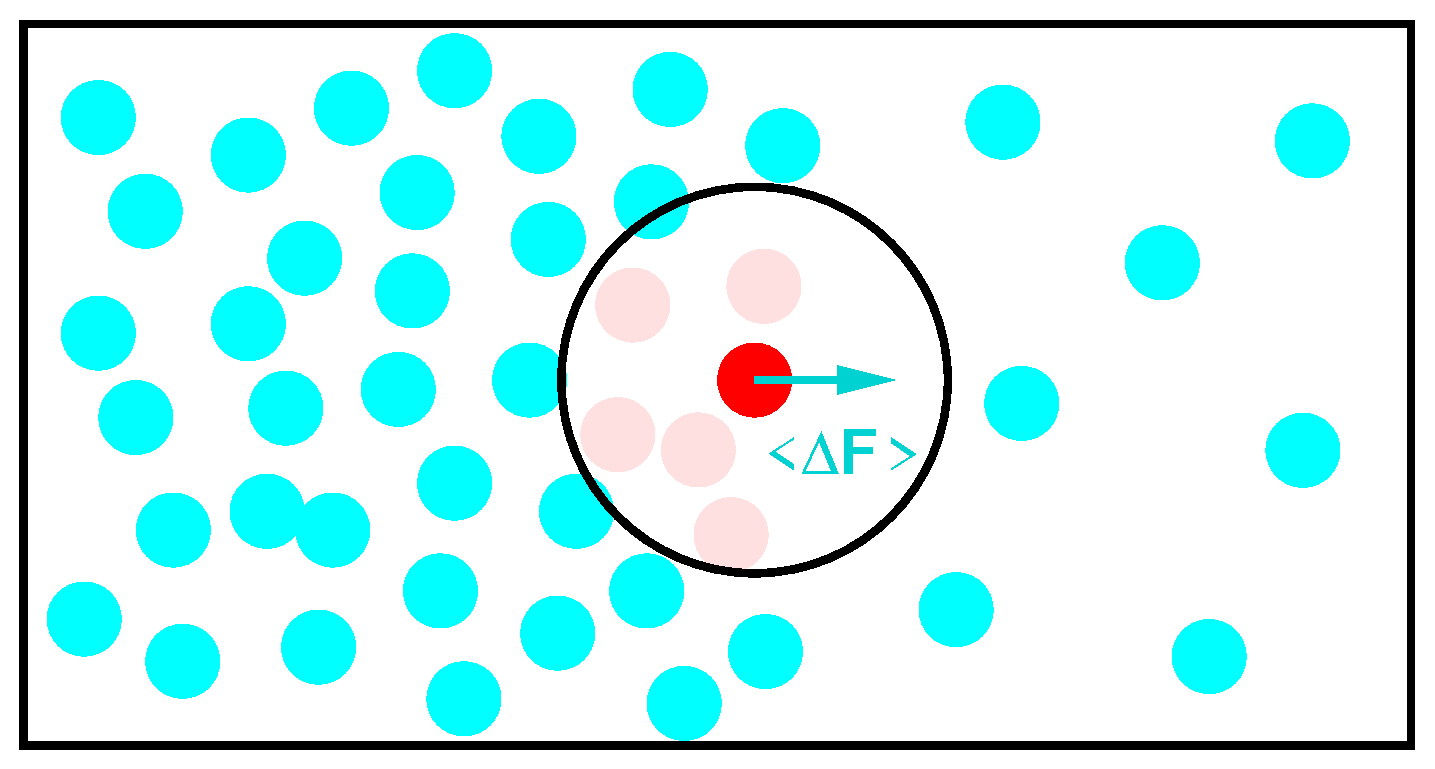
\includegraphics[width=0.9\textwidth]{figs/t0.85-n16000-rc07.5uni/cut-interface-step05.eps}
  \end{figure}  
\end{frame}

\begin{frame}{Long-range force correction}
  \begin{itemize}\itemsep -10pt
  \item<1-> Force correction:
    \bluec{
      \begin{align*}
        \vect F_{\textrm{corr}}(\vect r) =
        {\vect F}_{\textrm{calculated}}(\vect r) +
        \redc{\langle\Delta\vect F(\vect r)\rangle}.
      \end{align*}}
  \item<2->   The mean of
    the corrected error force vanishes:
    \bluec{
      \begin{align*}
        \langle\Delta\vect F_{\textrm{corr}}(\vect r)\rangle
        =
        \big\langle\,
        \vect F_{\textrm{exact}}(\vect r) - {\vect F}_{\textrm{calculated}}(\vect r) - \langle\Delta\vect F(\vect r)\rangle\,
        \big\rangle = 0.
      \end{align*}}
  \item<3-> The mean square error is given by
    \bluec{
      \begin{align*} \nonumber
        \langle\vert\Delta\vect F_{\textrm{corr}}(\vect r)\vert^2\rangle
        =
        \redc{\mathcal E^2_{\textrm{homo}}(\vect r)} +
        \redc{\mathcal E_{\textrm{correlation}}(\vect r)}.
      \end{align*}}
    which contains \redc{NO} inhomogeneous part.
  \end{itemize}
\end{frame}

\begin{frame}{Long-range force correction}
  \begin{figure}
    \centering
    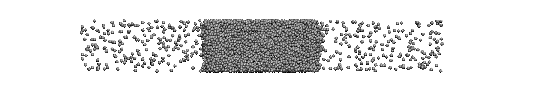
\includegraphics[scale=1]{figs/t0.85-n16000-rc07.5uni/confout-02.eps}\\
    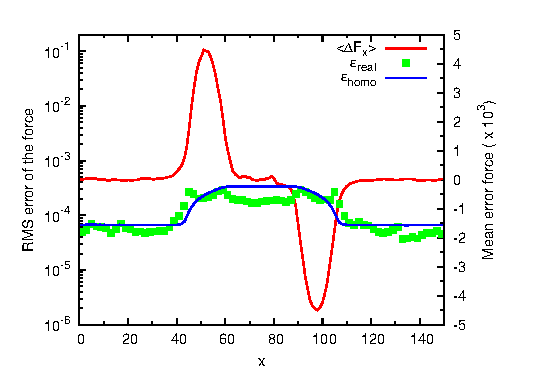
\includegraphics[]{figs/t0.85-n16000-fcorr-rc07.5-feq0200/fcorr-and-error.eps}
  \end{figure}
\end{frame}

\begin{frame}{Adaptive cut-off radius}
  \begin{figure}
    \centering
    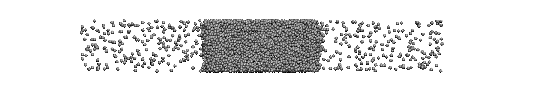
\includegraphics[scale=1]{figs/t0.85-n16000-rc07.5uni/confout-02.eps}\\
    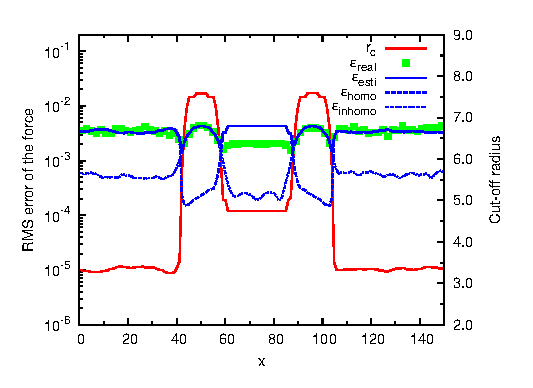
\includegraphics[]{figs/t0.85-n16000-adapt-e0.0045-extend/rcut-and-error.eps}
  \end{figure}
\end{frame}



\renewcommand\arraystretch{1.1}
\begin{frame}{Accuracy and efficiency}
  \begin{table}
  \centering
  \begin{tabular*}{0.8\textwidth}{c|@{\extracolsep{\fill}}lcc}\hline\hline
    $r^\ast_{c}$ & \textrm{method} & $\max\mathcal E^\ast$ & Cost($\times 10^{-6}$) \\ \hline
     &\textrm{uniform} & $8.6\times 10^{-2}$ & 2.9 \\
 3.5 &\textrm{adaptive} & $8.6\times 10^{-2}$ & 1.9 \\
     &\textrm{force corr} & $1.4\times 10^{-2}$ & 3.1 \\\cline{1-4}
     &\textrm{uniform} & $2.2\times 10^{-2}$ & 7.8 \\
 5.0 &\textrm{adaptive} & $2.2\times 10^{-2}$ & 4.5 \\
     &\textrm{force corr} & $1.9\times 10^{-3}$ & 7.9 \\\cline{1-4}
 6.0 &\textrm{uniform} & $1.1\times 10^{-2}$ & 13 \\\cline{1-4}
     &\textrm{uniform} & $4.5\times 10^{-3}$ & 24 \\
 7.5 &\textrm{adaptive} & $4.3\times 10^{-3}$ & 12 \\
     &\textrm{force corr} & $2.3\times 10^{-4}$ & 24 \\\cline{1-4}
     &\textrm{uniform} & $1.4\times 10^{-3}$ & 53 \\
10.0 &\textrm{adaptive} & $1.4\times 10^{-3}$ & 26 \\
     &\textrm{force corr} & $5.3\times 10^{-5}$ & 53 \\ \hline\hline
  \end{tabular*}
\end{table}
\end{frame}
\renewcommand\arraystretch{1.5}


\begin{frame}{Equilibrium gas density}
  \begin{figure}
    \centering
    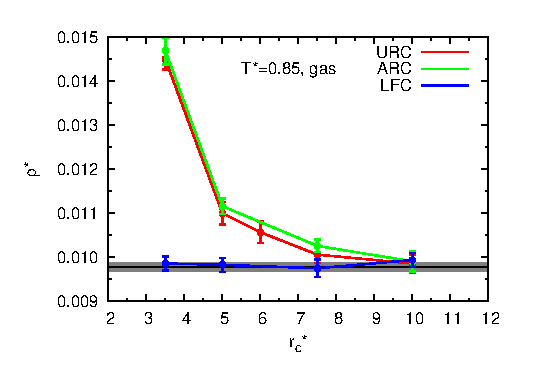
\includegraphics[]{figs/converge.new/t0p85-gas.eps} 
  \end{figure}
  URC: uniform cut-off, ARC: adaptive cut-off, LFC: long-range force correction.
\end{frame}

\begin{frame}{Equilibrium liquid density}
  \begin{figure}
    \centering
    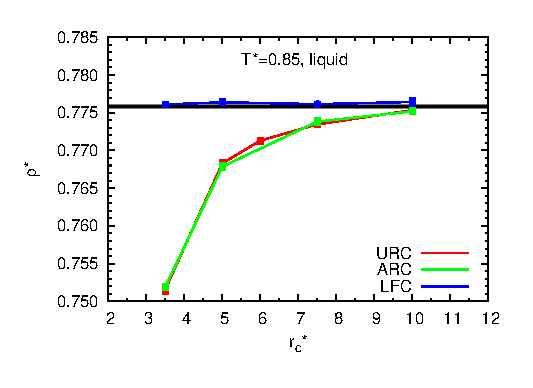
\includegraphics[]{figs/converge.new/t0p85-liquid.eps} 
  \end{figure}
  URC: uniform cut-off, ARC: adaptive cut-off, LFC: long-range force correction.
\end{frame}


\begin{frame}{Surface tension}
  \begin{figure}
    \centering
    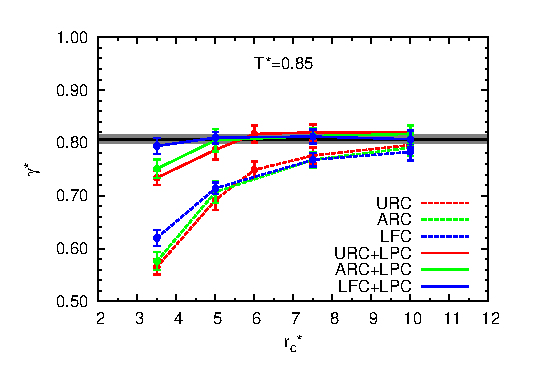
\includegraphics[]{figs/converge.new/tension-t0p85.eps} 
  \end{figure}
  URC: uniform cut-off, ARC: adaptive cut-off, LFC: long-range force correction,
  LPC: long-range pressure correction.
\end{frame}


% \begin{frame}{Conclusion of the cut-off method}
%   \centerline{\redc{The inhomogeneity error is bad}}.
% \end{frame}


\begin{frame}{Electrostatic interaction and Ewald summation}
  \begin{itemize}
  \item<1->   Electrostatic interaction:
  \begin{equation*}\bluec{
    U_{\textrm{ele}} = \frac12 \sum^\ast_{n}\sum_{i,j}\frac{q_i q_j}{\vert \vect r_{ij} + \vect n\vert}}
  \end{equation*}
\item <2->
  Ewald summation (1921) splits the
  energy into three parts
  \bluec{
  \begin {align*}
    U_{\textrm{ele}} &=  U_{\textrm{dir}} + U_{\textrm{rec}}+ U_{\textrm{corr}}\\
    U_{\textrm{dir}} & = \frac12 \sum^{\ast}_{\vect n}
    \sum_{i,j = 1}^{N} \frac{q_iq_j\, \redc{\textrm{erfc}(\beta \vert\vect{r}_{ij} + \vect{n}\vert)}}
    {\vert\vect{r}_{ij} + \vect{n}\vert} \\ \label{Erec-ewald}
    U_{\textrm{rec}} & = \frac1{2\pi V} \sum_{\vect m \neq 0}
    \frac{\redc{\exp(-\pi^2\vect m^2 / \beta^2)}}{\vect m^2} S(\vect m) S(-\vect m) \\
    U_{\textrm{corr}}& = -\frac\beta{\sqrt \pi} \sum_{i=1}^N q_i^2
  \end {align*}}
  \end{itemize}
\end{frame}


\begin{frame}{Smooth Particle Mesh Ewald Method (SPME)}{Basic concepts}
  \begin{itemize}\itemsep -5pt
  \item<1-> The structure factor \bluec{$S(\vect m)$} is
    defined by \bluec{
      \begin{equation*}\label{sm1}
        S(\vect m) = \sum_{j=1}^N q_j \exp (2 \pi i \vect m \cdot \vect r_j),
      \end{equation*}}
  \item<2-> Optimal computational cost\footnote{
    \bluec{J. Perram, H. Petersen and S. De Leeuw, Mol. Phys. \textbf{65}, 875 (1988).}}: \redc{$\mathcal O(N^{1.5})$}.
    \vskip .5cm
  \item<3-> \redc{SPME}\footnote{
    \bluec{U. Essmann, \textit{et. al.}, J. Chem. Phys. \textbf{103}, 8577 (1995).}}: interpolate \bluec{$S(\vect m)$} on grid, then FFT.
    The computational cost is 
  \begin{align*}
    \begin{tabular}[t]{c}
      \redc{$\mathcal O(N)$}\\
      {direct}
    \end{tabular}
    +
    \begin{tabular}[t]{c}
      \redc{$\mathcal O(N)$}\\
      {interpolation}
    \end{tabular}
    +
    \begin{tabular}[t]{c}
      \redc{$\mathcal O(N\log N)$}\\
      {FFTs}
    \end{tabular}
    =
    \begin{tabular}[t]{c}
      \redc{$\mathcal O(N\log N)$}\\
      {total cost}
    \end{tabular}
    \end{align*}
  \end{itemize}
\end{frame}

\begin{frame}{Smooth Particle Mesh Ewald Method (SPME)}
  {The working parameters is 6 dimensional}
  \vfill
  To use SPME method, one should provide the following parameters.
  \vfill
  \begin{itemize}
    \item \redc{$\beta$} \quad The controlling parameter.
    \item \redc{$r_c$} \quad The direct space cut-off radius.
    \item \redc{$\vect K$} \quad The reciprocal space cut-off. The number of FFT grid points.
    \item \redc{$n$} \quad The order of cardinal B-spline interpolation.
  \end{itemize}
  \vfill An arbitrary combination may lead to \redc{totally wrong
    results}.
  \vfill
  Two branches of force derivation: ik- and ananlytical differentiation.
  \vfill
\end{frame}

\begin{frame}{Long-range, homogeneous, uncorrelated}
  \begin{enumerate}\itemsep 3pt
  \item {Homogeneous}.
  \item Particles are {uncorrelated}.
  \end{enumerate}
    \begin{table}
    \centering
    \begin{tabular*}{0.85\textwidth}{l@{\extracolsep{\fill}}ll}\hline\hline
      Conditions & cut-off & SPME \\\hline
      1+2 & \shadowc{\tickYes\quad$\mathcal O(1)$}  & \bluec{\tickYes\quad$\mathcal O(1)$} \\
      2   & \shadowc{\tickYes\quad$\mathcal O(N\log N)$} & \shadowc{\tickYes\quad$\mathcal O(N\log N)$} \\
      none& \shadowc{\tickNo\quad$\mathcal O(N^2\log N)$} & \shadowc{\tickNo\quad$\mathcal O(N^2\log N)$} \\
          &  & \shadowc{N.N.A. $\mathcal O(N\log N)$} \\\hline\hline
    \end{tabular*}
  \end{table}
\end{frame}

\begin{frame}{Long-range, homogeneous, uncorrelated}
  \begin{figure}
  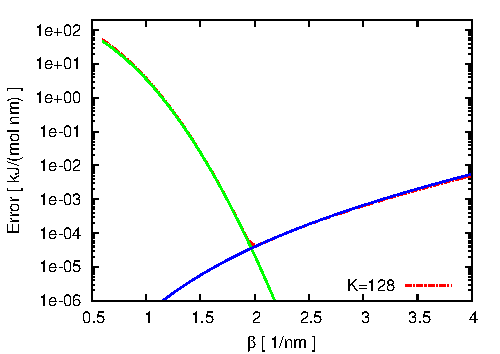
\includegraphics[width=0.7\textwidth]{figs/long-range//bspline-order6.pdf}
\end{figure}
  The SPME error estimate\footnote{
    \bluec{H. Wang, F. Dommert and C. Holm, J. Chem. Phys. \textbf{133}, 034117 (2010).}}
  is available in MD package Gromacs \redc{now}.
\end{frame}


% \begin{frame}{The parameter tuning of SPME }
%   The parameter tuning is a constrained optimization problem:\footnote{
%     \bluec{H. Wang, F. Dommert and C. Holm, J. Chem. Phys. \textbf{133}, 034117 (2010).}}
%   \bluec{
%     \begin{align*} 
%       \min\quad &  T (r_c, \vect K, n, \beta),\\
%       \textrm{\textbf{s.t.}}\quad & \mathcal E (r_c, \vect K, n, \beta) = \mathcal E_{\textrm{C}}
%     \end{align*}}
%   \redc{Nearly optimal} working parameters can be found \redc{automatically}.
% \end{frame}


\begin{frame}{Long-range, inhomogeneous, correlated}
  \begin{enumerate}\itemsep 3pt
  \item {Homogeneous}.
  \item Particles are {uncorrelated}.
  \end{enumerate}
    \begin{table}
    \centering
    \begin{tabular*}{0.85\textwidth}{l@{\extracolsep{\fill}}ll}\hline\hline
      Conditions & Short-range & Long-range \\\hline
      1+2 & \shadowc{\tickYes\quad$\mathcal O(1)$}  & \shadowc{\tickYes\quad$\mathcal O(1)$} \\
      2   & \shadowc{\tickYes\quad$\mathcal O(N\log N)$} & \redc{\tickYes\quad$\mathcal O(N\log N)$} \\
      none& \shadowc{\tickNo\quad$\mathcal O(N^2\log N)$} & \shadowc{\tickNo\quad$\mathcal O(N^2\log N)$} \\
          &  & \shadowc{N.N.A. $\mathcal O(N\log N)$} \\\hline\hline
    \end{tabular*}
  \end{table}
\end{frame}


\begin{frame}{The inhomogeneity error of SPME}
  \begin{itemize}
  \item <1-> The error kernels are available
    for \redc{Ewald summation}, \redc{SPME} and \redc{staggered mesh SPME}.
  \item <1-> The mean error force is
    \bluec{
      \begin{align*}
        \langle\Delta\vect F(\vect r)\rangle
        =
        q\int_{\mathbb R^3}\vect K(\vect r , \vect r')\,\rho_q(\vect r')\,\d d\vect r'
      \end{align*}
    }
    with
    \begin{align*}
      \bluec{  \rho_q(\vect r) = 
        \bigg\langle
        \sum_{j = 1}^N
        q_j\delta(\vect r - \vect r_j)
        \bigg\rangle
      }
    \end{align*}    
    Varnishes if the system is \redc{locally neutral}.
  \end{itemize}
\end{frame}


\begin{frame}{Error estimate in an inhomogeneous and uncorrelated system}
  \begin{figure}
    \centering
    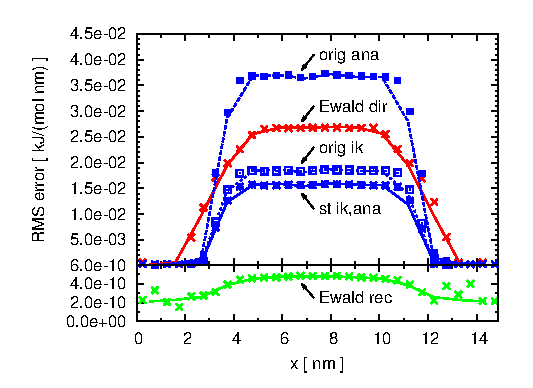
\includegraphics[width=0.9\textwidth]{figs/long-range-inhomo/rand1-error.eps}
  \end{figure}  
\end{frame}


\begin{frame}{Long-range, inhomogeneous, correlated}
  \begin{enumerate}\itemsep 3pt
  \item {Homogeneous}.
  \item Particles are {uncorrelated}.
  \end{enumerate}
    \begin{table}
    \centering
    \begin{tabular*}{0.85\textwidth}{l@{\extracolsep{\fill}}ll}\hline\hline
      Conditions & Short-range & Long-range \\\hline
      1+2 & \shadowc{\tickYes\quad$\mathcal O(1)$}  & \shadowc{\tickYes\quad$\mathcal O(1)$} \\
      2   & \shadowc{\tickYes\quad$\mathcal O(N\log N)$} & \shadowc{\tickYes\quad$\mathcal O(N\log N)$} \\
      none& \shadowc{\tickNo\quad$\mathcal O(N^2\log N)$} & \redc{\tickNo\quad$\mathcal O(N^2\log N)$} \\
          &  & \redc{N.N.A. $\mathcal O(N\log N)$} \\\hline\hline
    \end{tabular*}
  \end{table}
\end{frame}



\begin{frame}{The trouble in the inhomogeneous water system}
  {Staggered mesh SPME}
  \begin{figure}
    \centering
    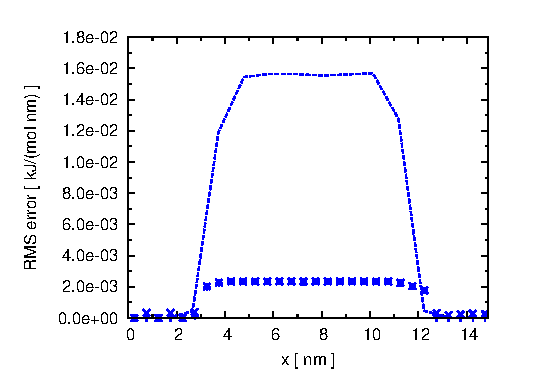
\includegraphics[width=0.9\textwidth]{figs/long-range-inhomo/water-st-error-1.eps}
  \end{figure}  
\end{frame}

\begin{frame}{The correlations in a water system}{Radial distribution functions}
  \begin{figure}
    \centering
    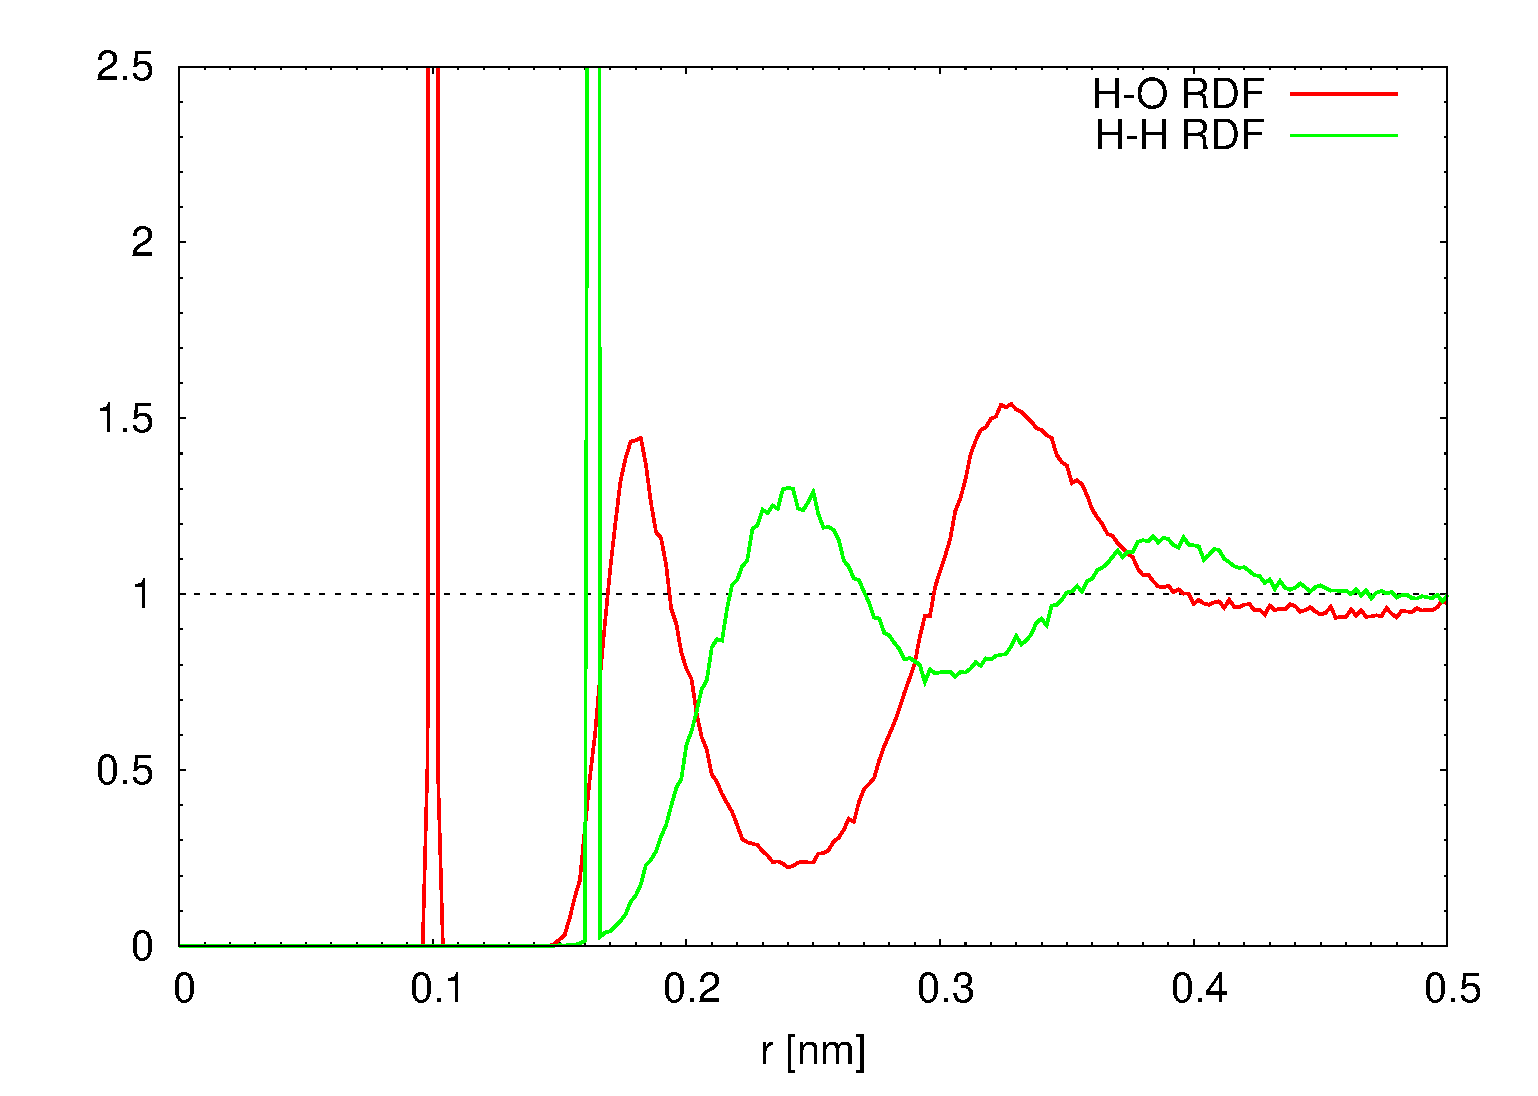
\includegraphics[width=0.8\textwidth]{figs/long-range-nna/rdf-corr-h2o-0.eps}
  \end{figure}
\end{frame}

\begin{frame}{The correlations in a water system}{Radial distribution functions}
  \begin{figure}
    \centering
    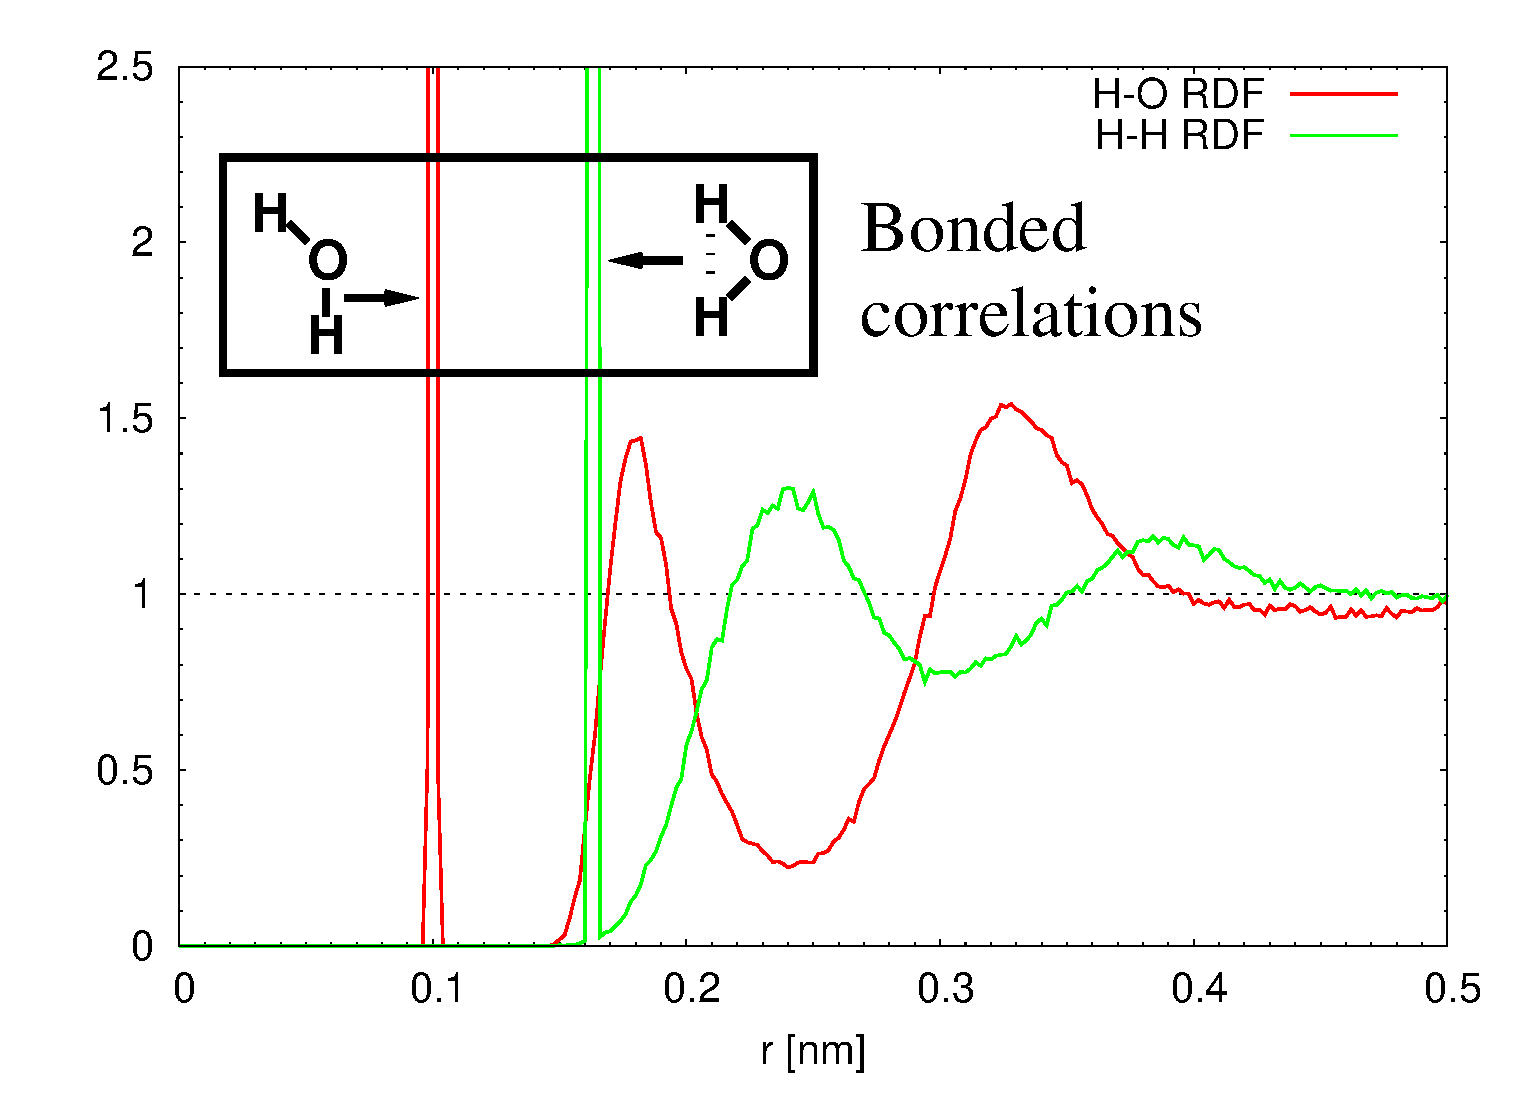
\includegraphics[width=0.8\textwidth]{figs/long-range-nna/rdf-corr-h2o-1.eps}
  \end{figure}
\end{frame}


\begin{frame}{Nearest neighbor approximation of the correlation error}{Staggered mesh SPME}
  \begin{figure}
    \centering
    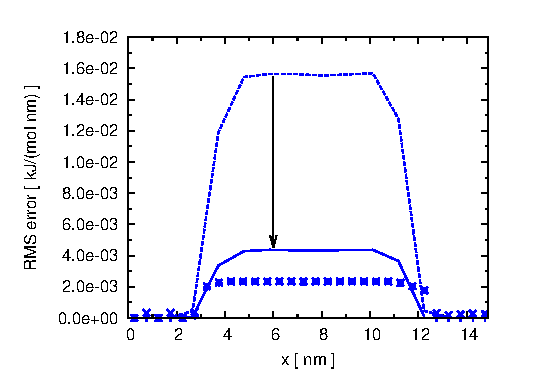
\includegraphics[width=0.9\textwidth]{figs/long-range-inhomo/water-st-error-2.eps}
  \end{figure}  
\end{frame}

\begin{frame}{The correlations in a water system}{Radial distribution functions}
  \begin{figure}
    \centering
    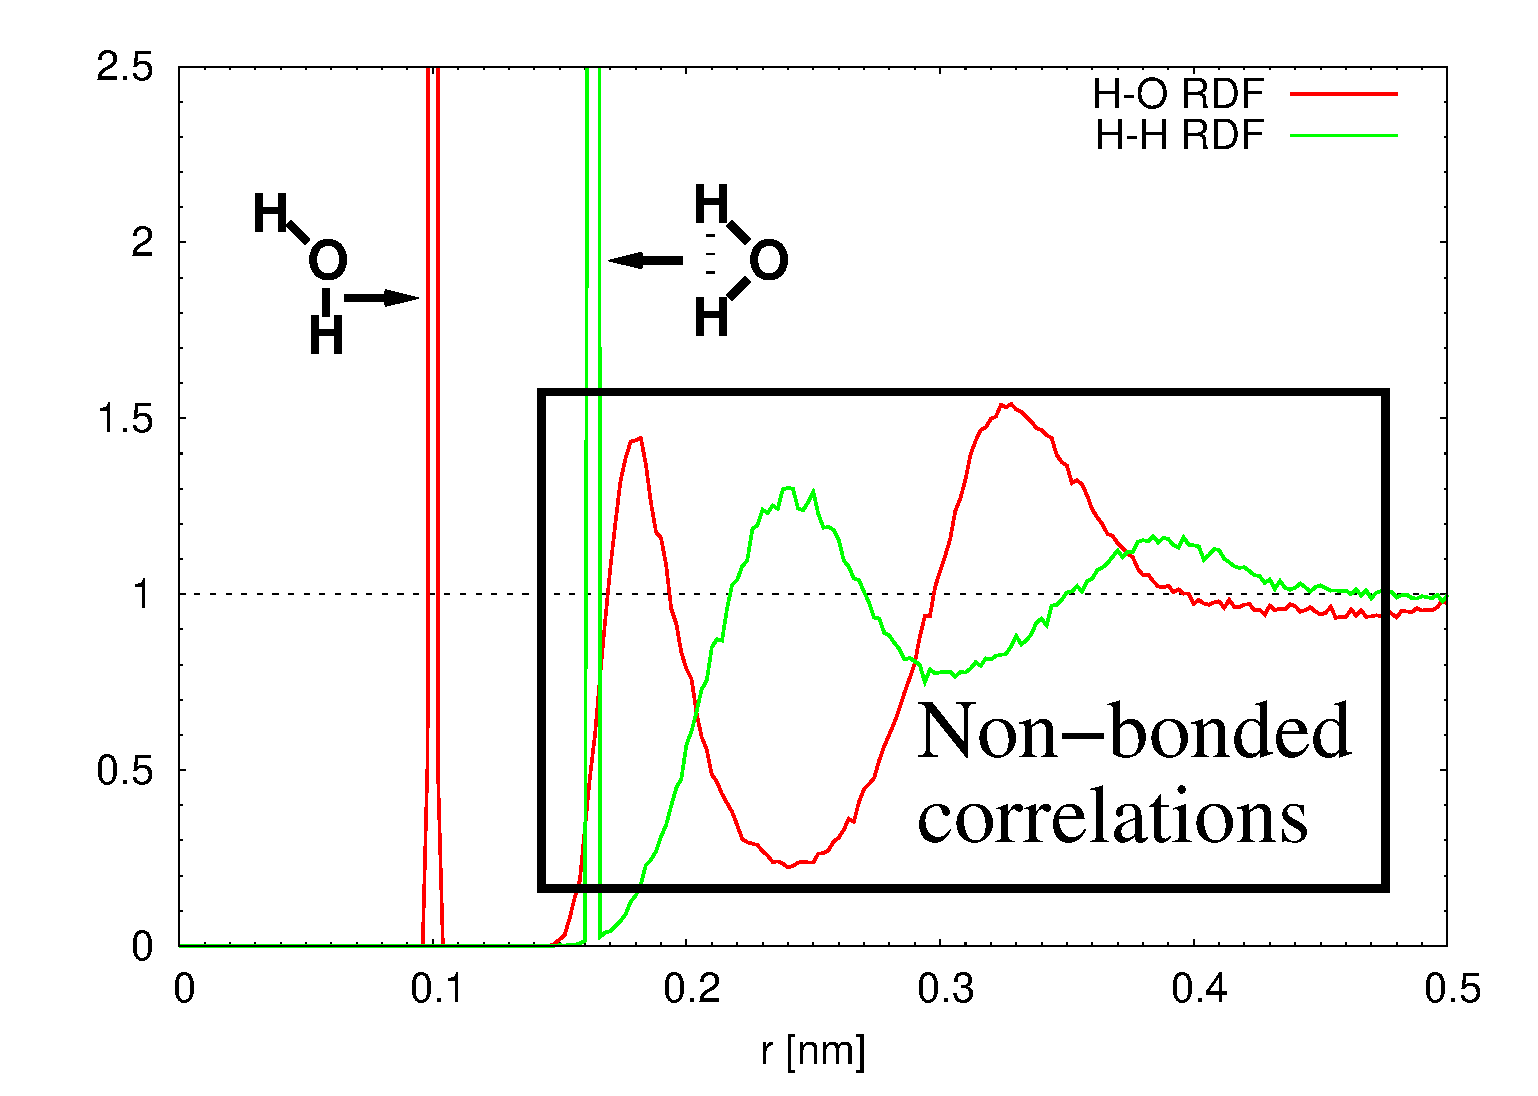
\includegraphics[width=0.8\textwidth]{figs/long-range-nna/rdf-corr-h2o-gr.eps}
  \end{figure}
\end{frame}


\begin{frame}{Nearest neighbor approximation of the correlation error}{Staggered mesh SPME}
  \begin{figure}
    \centering
    \includegraphics[width=0.9\textwidth]{figs/long-range-inhomo/water-st-error-3.eps}
  \end{figure}  
\end{frame}

% \begin{frame}{Summary}
%   \begin{itemize}
%   \item 
%   \end{itemize}
% \end{frame}

\begin{frame}
  \vfill
  \centerline{ \Huge
    Thanks!  }
  \vfill
  \bluec{
    \begin{align*} \nonumber
      \langle\vert\Delta\vect F(\vect r)\vert^2\rangle
      = 
      \redc{\mathcal E^2_{\textrm{homo}}(\vect r)} +
      % \langle\Delta\vect F(\vect r)\,\rangle^2 +
      \redc{\mathcal E^2_{\textrm{inhomo}}(\vect r)} +
      \redc{\mathcal E_{\textrm{correlation}}(\vect r)}.
    \end{align*}
  }
\end{frame}


\end{document}
